\section{Aufbau der Lösung}\label{sec:01_02_aufbauLoesung}
Das Projekt zur Entwicklung eines graphbasierten Informationssystem für die Analyse sozialer Interaktionen im Deutschen Bundestag, welches \glqq Sentiments Of Bundestag\grqq{} genannt wurde, besteht, wie bereits erwähnt, aus sieben Teilprojekten. Im folgenden Abschnitt wird grob auf die Thematiken der einzelnen Gruppen eingegangen.

\begin{figure}[H]
    \centering
    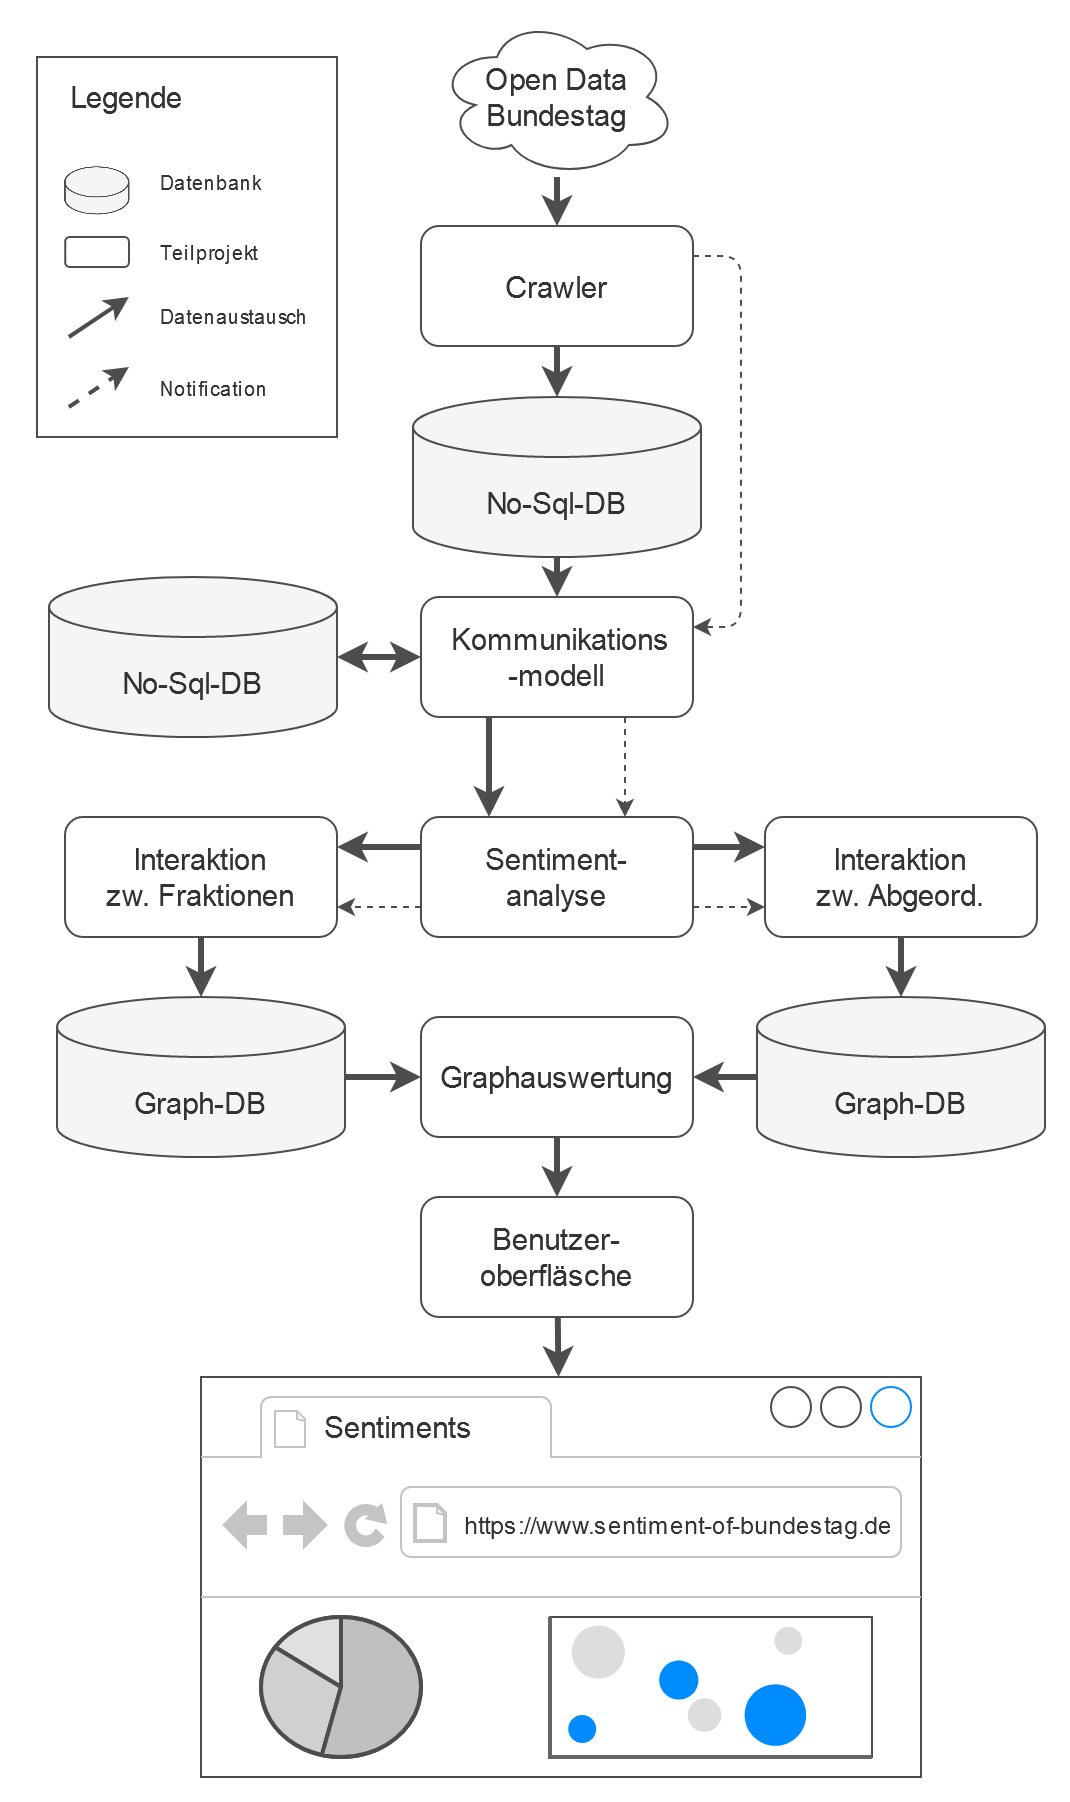
\includegraphics[width=\textwidth]{images/01-Einleitung/SentimentOfBundestag.png}
    \caption{Aufbau der Lösung}
    \label{fig:aufbauderLösungSOB}
\end{figure}
Die auf der Abbildung~\ref{fig:aufbauderLösungSOB} dargestellten Teilprojekten sind hier nun detaillierter aufgelistet:
\begin{itemize}
  \item \textbf{Crawler}: Scannt regelmäßig die Open Data Webseite des Bundestags, sucht, parst und speichern neue Protokollen sowie Stammdaten der Abgeordneten in seiner No-Sql-Datenbank. Ziel ist es hier sicherzustellen, das die DB immer auf dem neusten Stand bleibt
  \item \textbf{Kommunikationsmodell}: Analysiert und erstellt aus den Protokollen von Gruppe 1 ein Kommunikationsmodell aus den Austauschen im Bundestag
  \item \textbf{Sentiment-Analyse}: Sentiment Analysis (Stimmungsanalyse). Ziele sind hier die Identifikation der Stimmung in den Äußerungen der Abgeordneten und die Verrechnung der Stimmung einer Äußerung zu positiver/negativer Bewertung der Beziehung
  \item \textbf{Interaktion zwischen Abgeordneten}: Aus dem Kommunikationsmodell von Gruppe 2 und die Stimmungsanalyse von Gruppe 3 werden hier Interaktionen zwischen einzelnen Personen (Abgeordneten, Präsident, Gäste, etc.) identifiziert. Erstellt wird hier ein gewichteter Sentiment-Graph zwischen Abgeordneten mit positiven/negativen Gewichtungen
  \item \textbf{Interaktion zwischen Fraktionen}: Aus dem Kommunikationsmodell von Gruppe 2 und den Sentiment-Graph zwischen Personen von Gruppe 4 werden hier Interaktionen zwischen Gruppen von Personen analysiert und in einen Sentiment-Graph zwischen Parteien. Der besteht aus einer Aggregation der Abgeordnetensentiments zu gewichteten Sentiment-Graph der Parteien (Fraktionen, Gruppen, etc.)
  \item \textbf{Graphauswertung}: Die Sentiment-Graphen von den Gruppen 4 und 5 werden hier anhand verschiedener Auswertungsmethoden analysiert und die Ergebnisse davon die nächste Gruppe (Benutzeroberfläche) zur Verfügung stellt. 
  \item \textbf{Benutzeroberfläche}: Ziel ist hier die Realisierung einer interaktiven Benutzeroberfläche zur Darstellung der ausgewerteten Ergebnisse
\end{itemize}

Die einzelnen Teilprojekten werden in den nächsten Kapiteln in dieser Reihenfolge dokumentiert. 